\section{Overview}
\begin{itemize}
    \item Debugging is the process of finding and fixing errors in a program, usually logic or compiler/syntax errors.
    \item For syntax errors, understand what the compiler is telling you. 
    \item For always focus on fixing the first problem detected. 
    \item Debugging can vary in complexity. 
    \item It's a tremendous skill for programming. 
    \item Debugging saves time and money.
    \item Maintenance phase is the most expensive phase of the software life cycle, when windows releases a new operating system they have the responsibility to fix bugs that may arise, this is why automatic updates are pushed to you computer sometimes. 
    \item Understand, bugs are unavoidable, it's ok. 
\end{itemize}
\subsection{Common problems}
\begin{itemize}
    \item Logical errors: it compiles but it doesn't function as intended, example: having a loop do more iterations as it is intended. These are caught by the programmer on execution.
    \item Syntax errors: errors related to not following the rules of the language, example: not putting a semi-colon at the end of a statement. These are caught by the compiler.
    \item Memory corruption: not freeing memory can lead to this. 
        \begin{itemize}
            \item Memory not being used 
            \item Memory leeks 
            \item Dangling references
        \end{itemize}
    
    \item Performance / Scalability: as the users or features become greater in number, the app crashes. 
    \item Lack of cohesion: a function is doing too much, areas not used. 
    \item Tight coupling (dependencies): your algorithm is dependent on a lot of things. 
\end{itemize}
In writing code, you always want to strive for high cohesion and low coupling. 

\subsection{Debugging process}
\begin{itemize}
    \item Understand the problem: test, understand requirements. 
    \item Reproduce the problem: 
        \begin{itemize}
            \item Sometimes very difficult as problems can be intermittent or only happen in very rare circumstances. 
            \item Parallel process or threading problems. 
        \end{itemize}
    
    \item Simplify the problem / divide and conquer / isolate the source.
        \begin{itemize}
            \item Remove parts of the original test case. 
            \item Comment out the code / back out changes 
            \item Turn a large program into a lot of small programs (unit testing).
        \end{itemize}
    
    \item Identify origin of the problem (in the code):
        \begin{itemize}
            \item Use debugging tools if necessary. 
        \end{itemize}
    
    \item Solve the problem: 
        \begin{itemize}
            \item Experience and practice 
            \item Sometimes includes redesign or refactor of code. 
            \item Test like crazy, verify. 
        \end{itemize}
\end{itemize}

\subsection{Techniques and tools}
\begin{itemize}
    \item Tracing / using print statements:
        \begin{itemize}
            \item Output values of variables at certain points of a program 
            \item Show the flow of execution 
        \end{itemize}
    
    \item Debuggers: monitor the execution of a program, stop it, restart it, set breakpoints and watch variables in memory.
    \item Log files: can be used for analysis, add ``good'' log statements to your code, useful for un-reproducible bugs. 
    \item Monitoring software: tun-time analysis of memory usage, network traffic, thread and object information. 
    \item Exception handling: C doesn't support that. 
    \item Static analyzers: analyze the source code for specific set of known problems, analyze the code without it running: 
        \begin{itemize}
            \item Semantic checker, does not analyze syntax.
            \item Can detect things like uninitialized variables, memory leaks, unreachable code, deadlocks or race condition. 
            \item It's the intellisense. 
        \end{itemize}
    
    \item Test suites: run a set of comprehensive system end-to-end tests.
    \item Debugging the program after it has crashed: 
        \begin{itemize}
            \item Analyze the call stacks 
            \item Analyze memory dump (core file generated)
        \end{itemize}    
\end{itemize}

\subsection{Preventing errors}
\begin{itemize}
    \item Writing high quality code. 
        \begin{itemize}
            \item Using good variable names 
            \item Using efficient implementations
        \end{itemize}
    \item Unit test: automatically executed when compiling:
        \begin{itemize}
            \item Helps avoid regression 
            \item Finds errors in new code before it is delivered 
            \item TDD (Test Driven Development)
            \item If you unit testing is very large, this is an indicator of poor quality code. 
        \end{itemize}
    
    \item Provide good documentation and proper planning (write down design on paper and utilize pseudo code).
    \item Work in steps and constantly test after each step.
        \begin{itemize}
            \item Avoid too many changes at once. 
            \item When making changes, apply them incrementally. Add one change, then test thoroughly before starting the next step.
            \item Helps reduce the possible sources of bogs, limits problem set.
        \end{itemize}
\end{itemize}


%----------------------------------------------------------------------------------------
\section{Understanding the call stack}
\begin{itemize}
    \item A stack trace (call stack) is generated whenever your app crashes because of a fatal error, a stack is a data structure, it's useful because you can see what steps your program took to end up crashing.
    \item A stack trace shows a list of function calls that lead to the error.
        \begin{itemize}
            \item Includes the filenames and line numbers of the code that cause the exception or error to occur. 
            \item Top of the stack contains the last call that caused the error (nested calls).
            \item Bottom of the stack contains the first call that started the chain of calls to cause the error. 
            \item You need to find the call in your application that is causing the crash.
            \item It contains the line and the function that produced the error. Useful information for debugging. 
        \end{itemize}
    
    \item A programmer can also dump the stack trace, if you know that an error is going to happen you can dump it.
    \item You can build your program for release or with debugging information.
\end{itemize}
\begin{figure}[H]
    \centering
    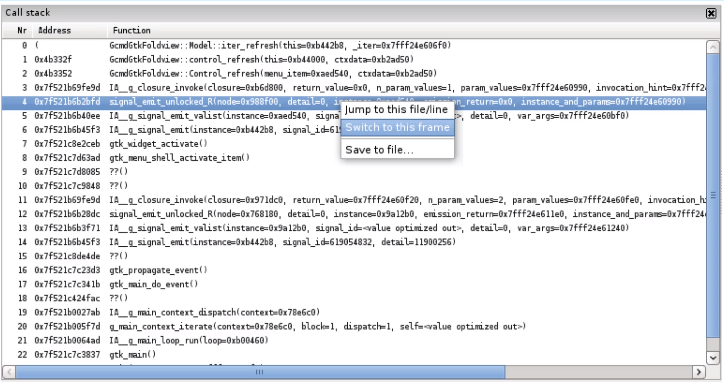
\includegraphics[width=15cm]{Figs/call_stack.png}  
\end{figure}
\begin{itemize}
    \item The question marks are unknown steps, on release builds the call stacks are empty, and in builds with debugging information they are populated, in releases this information is excluded so that the executable is lighter. 
\end{itemize}


%----------------------------------------------------------------------------------------
\section{Code blocks debugger}
\begin{itemize}
    \item Enable the -g flag 
    \item Disable optimization flags.
\end{itemize}


%----------------------------------------------------------------------------------------
\section{Common C mistakes}
\begin{itemize}
    \item Misplacing a semi-colon, example: \mintinline{c}{if (j == 100); j = 0;}, j will not be counted as part of the if statement. 
    \item Confusing the = with the == .
    \item Omitting function prototype declaration.
    \item Failing to include the header file that include the definition for a C-programming library function.
    \item Confusing a character constant and a character string. 
    \item Using the wrong bounds for an array. 
    \item Confusing the operator -> with the operator . when referencing structure members.
        \begin{itemize}
            \item The . is for structure variables.
            \item The -> is used for structure pointer variables.
        \end{itemize}
    \item Omitting the \& in scanf() for non-pointer variables.
    \item Using a pointer variable before it's initialized. 
    \item Omitting the break statement at the end of a case in a switch statement. 
    \item Inserting a semicolon at the end of a preprocessor definition.
    \item Omitting a closing parenthesis or closing quotation marks on any statement.
\end{itemize}


%----------------------------------------------------------------------------------------
\section{Understanding compiler errors and warnings}
\begin{itemize}
    \item Use the -Wall flag to turn everything on.
    \item The compiler will show two types of problems: errors and warnings. 
    \item In the -Wall flag will not allow you to compile the executable if there are any warnings. 
    \item Types of errors: 
        \begin{itemize}
            \item variable undeclared: not declaring a variable before using it. 
            \item warning: implicit declaration of function. You have not placed the function prototype. Or a warning appears saying that the function is used in the code but no previous information has been given about it.
            \item warning: control reaches end of non-void function: you forgot a return statement in a function. 
            \item warning: unused variable: variables not used. 
            \item undefined reference to ``'': linking is not posible because there is a function with no definition. 
            \item error: conflicting types: different function prototypes and function declarations.  
        \end{itemize}
    \item Run-time errors: 
        \begin{itemize}
            \item Array out of bounds, that are produced in run time. 
        \end{itemize}
    
    \item Google the error if you don't understand it. 
\end{itemize}
